

\tikzset{every picture/.style={line width=0.75pt}} %set default line width to 0.75pt        

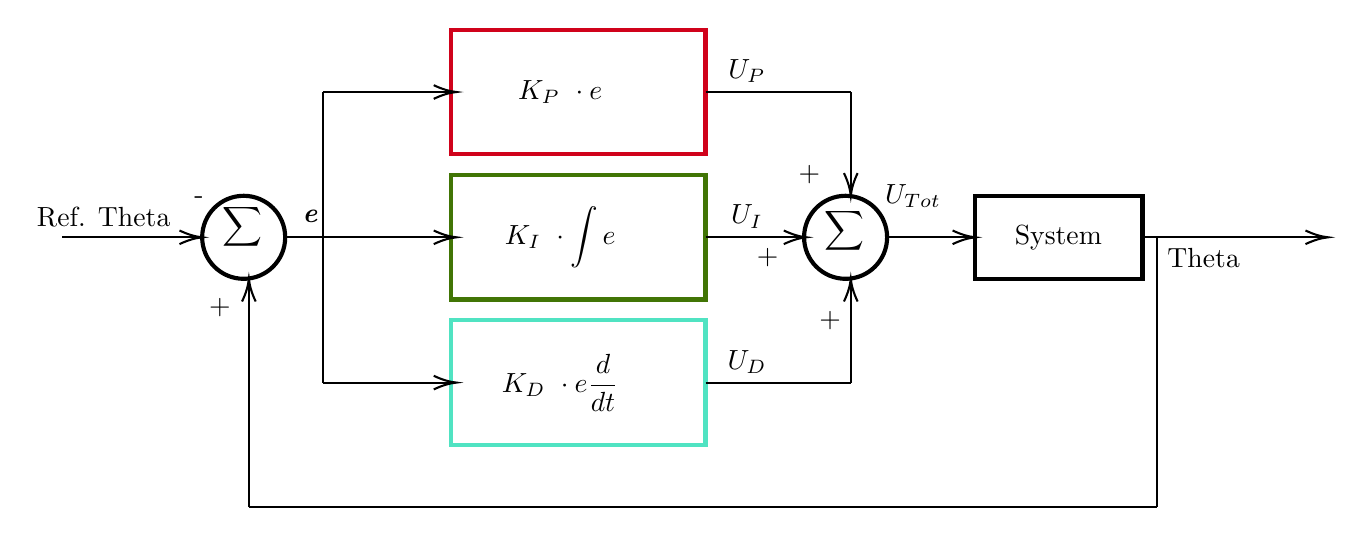
\begin{tikzpicture}[x=0.75pt,y=0.75pt,yscale=-1,xscale=1]
%uncomment if require: \path (0,269); %set diagram left start at 0, and has height of 269

%Shape: Rectangle [id:dp6186698400269734] 
\draw  [color={rgb, 255:red, 208; green, 2; blue, 27 }  ,draw opacity=1 ][line width=1.5]  (217.5,20) -- (340,20) -- (340,80) -- (217.5,80) -- cycle ;
%Shape: Rectangle [id:dp35497397654468] 
\draw  [color={rgb, 255:red, 65; green, 117; blue, 5 }  ,draw opacity=1 ][line width=1.5]  (217.5,90) -- (340,90) -- (340,150) -- (217.5,150) -- cycle ;
%Shape: Rectangle [id:dp0011241398633399236] 
\draw  [color={rgb, 255:red, 80; green, 227; blue, 194 }  ,draw opacity=1 ][line width=1.5]  (217.5,160) -- (340,160) -- (340,220) -- (217.5,220) -- cycle ;
%Shape: Circle [id:dp7081049529214984] 
\draw  [line width=1.5]  (97.5,120) .. controls (97.5,108.95) and (106.45,100) .. (117.5,100) .. controls (128.55,100) and (137.5,108.95) .. (137.5,120) .. controls (137.5,131.05) and (128.55,140) .. (117.5,140) .. controls (106.45,140) and (97.5,131.05) .. (97.5,120) -- cycle ;
%Straight Lines [id:da1012548517194285] 
\draw    (155.61,50) -- (218,50) ;
\draw [shift={(220,50)}, rotate = 180] [color={rgb, 255:red, 0; green, 0; blue, 0 }  ][line width=0.75]    (10.93,-3.29) .. controls (6.95,-1.4) and (3.31,-0.3) .. (0,0) .. controls (3.31,0.3) and (6.95,1.4) .. (10.93,3.29)   ;

%Straight Lines [id:da024552935574742696] 
\draw    (137.5,120) -- (218,120) ;
\draw [shift={(220,120)}, rotate = 180] [color={rgb, 255:red, 0; green, 0; blue, 0 }  ][line width=0.75]    (10.93,-3.29) .. controls (6.95,-1.4) and (3.31,-0.3) .. (0,0) .. controls (3.31,0.3) and (6.95,1.4) .. (10.93,3.29)   ;

%Straight Lines [id:da632489535879416] 
\draw    (155.61,190) -- (218,190) ;
\draw [shift={(220,190)}, rotate = 180] [color={rgb, 255:red, 0; green, 0; blue, 0 }  ][line width=0.75]    (10.93,-3.29) .. controls (6.95,-1.4) and (3.31,-0.3) .. (0,0) .. controls (3.31,0.3) and (6.95,1.4) .. (10.93,3.29)   ;

%Straight Lines [id:da028164362822356237] 
\draw    (155.61,50) -- (155.61,110) ;


%Straight Lines [id:da1783990189247291] 
\draw    (155.61,110) -- (155.61,190) ;


%Shape: Ellipse [id:dp13776991374733094] 
\draw  [line width=1.5]  (387.5,120) .. controls (387.5,108.95) and (396.45,100) .. (407.5,100) .. controls (418.55,100) and (427.5,108.95) .. (427.5,120) .. controls (427.5,131.05) and (418.55,140) .. (407.5,140) .. controls (396.45,140) and (387.5,131.05) .. (387.5,120) -- cycle ;
%Straight Lines [id:da5590648239872058] 
\draw    (340,50) -- (410,50) ;


%Straight Lines [id:da32339100567036794] 
\draw    (340,120) -- (386.65,120) ;
\draw [shift={(388.65,120)}, rotate = 180] [color={rgb, 255:red, 0; green, 0; blue, 0 }  ][line width=0.75]    (10.93,-3.29) .. controls (6.95,-1.4) and (3.31,-0.3) .. (0,0) .. controls (3.31,0.3) and (6.95,1.4) .. (10.93,3.29)   ;

%Straight Lines [id:da37714274354973676] 
\draw    (340,190) -- (410,190) ;


%Straight Lines [id:da12414839144602552] 
\draw    (410,50) -- (410,98) ;
\draw [shift={(410,100)}, rotate = 270] [color={rgb, 255:red, 0; green, 0; blue, 0 }  ][line width=0.75]    (10.93,-3.29) .. controls (6.95,-1.4) and (3.31,-0.3) .. (0,0) .. controls (3.31,0.3) and (6.95,1.4) .. (10.93,3.29)   ;

%Straight Lines [id:da2294854556231043] 
\draw    (410,142) -- (410,190) ;

\draw [shift={(410,140)}, rotate = 90] [color={rgb, 255:red, 0; green, 0; blue, 0 }  ][line width=0.75]    (10.93,-3.29) .. controls (6.95,-1.4) and (3.31,-0.3) .. (0,0) .. controls (3.31,0.3) and (6.95,1.4) .. (10.93,3.29)   ;
%Straight Lines [id:da7636925489142845] 
\draw    (427.5,120) -- (468,120) ;
\draw [shift={(470,120)}, rotate = 180] [color={rgb, 255:red, 0; green, 0; blue, 0 }  ][line width=0.75]    (10.93,-3.29) .. controls (6.95,-1.4) and (3.31,-0.3) .. (0,0) .. controls (3.31,0.3) and (6.95,1.4) .. (10.93,3.29)   ;

%Straight Lines [id:da8120471221631163] 
\draw    (30,120) -- (95.5,120) ;
\draw [shift={(97.5,120)}, rotate = 180] [color={rgb, 255:red, 0; green, 0; blue, 0 }  ][line width=0.75]    (10.93,-3.29) .. controls (6.95,-1.4) and (3.31,-0.3) .. (0,0) .. controls (3.31,0.3) and (6.95,1.4) .. (10.93,3.29)   ;

%Straight Lines [id:da7263862005723072] 
\draw    (120,250) -- (120,142) ;
\draw [shift={(120,140)}, rotate = 450] [color={rgb, 255:red, 0; green, 0; blue, 0 }  ][line width=0.75]    (10.93,-3.29) .. controls (6.95,-1.4) and (3.31,-0.3) .. (0,0) .. controls (3.31,0.3) and (6.95,1.4) .. (10.93,3.29)   ;

%Straight Lines [id:da9777886662003494] 
\draw    (120,250) -- (490,250) ;


%Shape: Rectangle [id:dp7284343716119925] 
\draw  [line width=1.5]  (470,100) -- (550.53,100) -- (550.53,140) -- (470,140) -- cycle ;
%Straight Lines [id:da4771680795774551] 
\draw    (550.53,120) -- (638,120) ;
\draw [shift={(640,120)}, rotate = 180] [color={rgb, 255:red, 0; green, 0; blue, 0 }  ][line width=0.75]    (10.93,-3.29) .. controls (6.95,-1.4) and (3.31,-0.3) .. (0,0) .. controls (3.31,0.3) and (6.95,1.4) .. (10.93,3.29)   ;

%Straight Lines [id:da7739849283065594] 
\draw    (557.37,120) -- (557.37,250) ;


%Straight Lines [id:da5629774692956326] 
\draw    (557.37,250) -- (485.79,250) ;



% Text Node
\draw (50,110) node  [align=left] {Ref. Theta};
% Text Node
\draw (510,120) node  [align=left] {System};
% Text Node
\draw (270,190) node  [align=left] {$\displaystyle K_{D} \ \cdot e  \frac{d}{dt}$};
% Text Node
\draw (270,120) node  [align=left] {$\displaystyle K_{I} \ \cdot \int e$};
% Text Node
\draw (270,50) node  [align=left] {$\displaystyle K_{P} \ \cdot e$};
% Text Node
\draw (390,90) node  [align=left] {+};
% Text Node
\draw (370,130) node  [align=left] {+};
% Text Node
\draw (400,160) node  [align=left] {+};
% Text Node
\draw (106,154) node  [align=left] {+};
% Text Node
\draw (96,101) node  [align=left] {\mbox{-}};
% Text Node
\draw (150,110) node  [align=left] {\textit{\textbf{e}}};
% Text Node
\draw (407,117) node  [align=left] {$\displaystyle \sum $};
% Text Node
\draw (360,110) node  [align=left] {$\displaystyle U_{I}$};
% Text Node
\draw (360,180) node  [align=left] {$\displaystyle U_{D}$};
% Text Node
\draw (360,40) node  [align=left] {$\displaystyle U_{P}$};
% Text Node
\draw (117,115) node  [align=left] {$\displaystyle \sum $};
% Text Node
\draw (440,100) node  [align=left] {$\displaystyle U_{Tot}$};
% Text Node
\draw (580,130) node  [align=left] {Theta};


\end{tikzpicture}
